\documentclass{article}


\usepackage{microtype}
\usepackage{graphicx}
\usepackage{subcaption}
\usepackage{booktabs} % for professional tables
\usepackage{multirow}
\usepackage{titlesec}

\usepackage{hyperref}
% Attempt to make hyperref and algorithmic work together better:
\newcommand{\theHalgorithm}{\arabic{algorithm}}

% Use the following line for the initial blind version submitted for review:
\usepackage[accepted]{icml2026}
\usepackage{amsmath}
\usepackage{amssymb}
\usepackage{mathtools}
\usepackage{amsthm}


% if you use cleveref..
\usepackage[capitalize,noabbrev]{cleveref}

%%%%%%%%%%%%%%%%%%%%%%%%%%%%%%%%
% THEOREMS
%%%%%%%%%%%%%%%%%%%%%%%%%%%%%%%%
\theoremstyle{plain}
\newtheorem{theorem}{Theorem}[section]
\newtheorem{proposition}[theorem]{Proposition}
\newtheorem{lemma}[theorem]{Lemma}
\newtheorem{corollary}[theorem]{Corollary}
\theoremstyle{definition}
\newtheorem{definition}[theorem]{Definition}
\newtheorem{assumption}[theorem]{Assumption}
\theoremstyle{remark}
\newtheorem{remark}[theorem]{Remark}

% Todonotes is useful during development; simply uncomment the next line
%    and comment out the line below the next line to turn off comments
%\usepackage[disable,textsize=tiny]{todonotes}
\usepackage[textsize=tiny]{todonotes}

\begin{document}

\twocolumn[
  \icmltitle{Evaluating the Structural Value of Knowledge Graphs with Text}

  \begin{icmlauthorlist}
    \icmlauthor{Matthew Krasnow}{}
    \icmlauthor{Seager Hunt}{}
    \icmlauthor{Reade Park}{}
    \icmlauthor{Cory Wu}{}
  \end{icmlauthorlist}

  \icmlkeywords{Machine Learning, ICML}

  \vskip 0.3in
]


\begin{abstract}
GraphRAG and structural-embedding methods broadly assume that graph structure carries predictive signal beyond what text alone provides. We test this assumption on PrimeKG, a 129{,}000-node biomedical knowledge graph, using cross-fit double machine learning (DML) to estimate the residual predictive value of structure for link prediction after partialling out a strong text baseline. We use four samplers as probes for distinct structural hypotheses (DeepWalk, node2vec-BFS, node2vec-DFS, GraphSAGE) and four schema-induced subgraphs spanning drug, gene/protein, pathway, disease, and phenotype contexts. Structure adds significant residual signal in all 16 (schema, sampler) combinations, but the magnitude anti-correlates with text-baseline strength. Under schema shift, walk-based samplers transfer universally while GraphSAGE fails, sometimes catastrophically (AUC drops $0.954 \rightarrow 0.768$); when text generalization collapses (text AUC $=0.474$), random-walk embeddings rescue prediction to AUC $\approx 0.93$. Walk-based structural embeddings encode schema-invariant biological primitives; aggregation-based features are schema-specific.
\end{abstract}

\section{Introduction}

Knowledge graphs have seen a surge of adoption across industry and academia, with notable usage at Google, Amazon, AirBNB, eBay, LinkedIn, and many others. This demonstrates their utility for integrating and extracting value from large, heterogeneous data at scale \citep{hogan2021}. Knowledge graphs use a graph-based abstraction to capture relations between entities in a way that is both concise and intuitive, as edges can encode connections that are inherent in social data, biological interactions, bibliographic citations, and more. Beyond simple relational structure, knowledge graphs can also contain rich textual descriptions assigned to their nodes, encode distinct types of edges representing different types of relations, and partition the nodes into heterogeneous categories. This makes them useful for complex domains where many kinds of entities interact through many kinds of relationships.

PrimeKG exemplifies this usefulness in the biomedical setting. It is a large precision medicine knowledge graph containing around 129,000 nodes and around 4 million relations between them. The nodes span 10 categories like gene, disease, drug, etc., and the edges span 29 categories like indication, interacts, side effect, drug carrier, etc. 

This diversity in node and edge types, while useful in the information it contains, it what makes graph learning on PrimeKG so challenging. Standard graph neural networks were designed for homogeneous graphs, and extending them to handle multiple node and edge types introduces substantial architectural and computational overhead. Heterogeneous GNNs must maintain separate parameters per relation type, making training expensive, which raises the question: is the structural overhead worth it?

In many recent systems, particularly retrieval-augmented generation pipelines, the answer has simply been no. These systems pass node text descriptions directly into a language model and ignore the graph entirely, making the assumption that the text content is sufficient. For knowledge graphs with rich node-level text, this assumption is not unreasonable, as two diseases that share similar clinical language are likely to share biological mechanisms, and this may be fully captured by text embeddings alone. If structure adds little beyond what text already encodes, then skipping the graph is computationally convenient. If the structure carries residual predictive signal through patterns of connectivity that the text does not explain, then ignoring it leaves information on the table. This paper investigates which of these regimes holds in PrimeKG \citep{primekg2023}, and under what biomedical contexts.

\section{Related Work}

\subsection{Graph Retrieval-Augmented Generation}

Retrieval-augmented generation has become a standard approach for grounding large language model outputs in external knowledge \citep{lewis2020rag}. Graph RAG extends this idea by leveraging relational structure to retrieve more contextually relevant information than text similarity alone. \citet{grag2024} introduce GRAG, which retrieves textual subgraphs around query-relevant entities via a divide-and-conquer strategy, then encodes them through complementary text and graph views before passing context to an LLM, demonstrating strong improvements on multi-hop reasoning benchmarks. \citet{stark2024} introduce STaRK, a benchmark for semi-structured retrieval over text-rich knowledge bases, which we use as our primary evaluation setting. A common assumption across GraphRAG systems is that combining text and structure improves over either alone, yet none of these works systematically isolates the residual contribution of structure after controlling for what text already encodes. Our work addresses this gap directly.

\subsection{Hybrid and Fidelity-Aware Retrieval}

Several recent systems have questioned whether GraphRAG methods actually retrieve what they claim to. \citet{mor2025} propose MoR (Mixture of Retrieval), which interweaves structural traversal and textual matching through a planning-reasoning-organizing framework, and note uneven performance across query types without characterizing the source of that unevenness. \citet{graphflow2025} critically examine retrieval fidelity in graph RAG, introducing GraphFlow and showing that existing methods frequently fail to surface relevant context, particularly for queries that require multi-hop relational reasoning. Both works motivate our question: before designing more sophisticated hybrid systems, it is worth asking how much structural information contributes beyond what node text already provides, and whether that contribution is consistent across different biomedical reasoning contexts.

\subsection{Text versus Structure in Graph Learning}

The question of whether graph structure adds information beyond node features has received attention in the graph machine learning literature, primarily in the context of node classification on homogeneous graphs. Several works have shown that for graphs with highly informative node features, message-passing GNNs offer limited improvement over feature-only baselines, with the benefit of structural aggregation depending heavily on the correlation between features and topology \citep{huang2023}. Heterogeneous graphs introduce additional complexity: with many node and edge types, learning meaningful structural representations requires handling combinatorial diversity in relation semantics, making it architecturally costly and unclear whether the overhead is justified. To our knowledge, no prior work applies a formal causal framework to isolate the residual value of graph structure on a biomedical knowledge graph with rich node-level text, controlling for the confounding correlation between textual and structural similarity. We fill this gap using Double Machine Learning \citep{dml2018} across multiple graph schemas and structural embedding strategies.

\section{Problem Formalization}

\textbf{Textual Graphs} are graphs consisting of text-attributed nodes and edges, which can be formally defined as $$G = (V, E, \{T_n\}_{n \in V}, \{T_e\}_{e\in E}).$$ $V$ and $E$ represent the node and edge set, and $T_n$ and $T_e$ represent natural language attributes of the corresponding nodes and edges in the graph. 

\textbf{Schemas} are subgraphs induced by restricting the graph $G$ to a set of node types $\mathcal{A}'$ and relation types $\mathcal{R}'$. Formally, 
$$
\mathcal{S}(G) = (V', E', \{T_n\}_{n \in V'}, \{T_e\}_{e \in E'}),
$$
where $V' = \{v \in V : \mathrm{type}(v) \in \mathcal{A}'\}$ and $E' = \{e=(u,v) \in E : u,v \in V' \text{ and } \mathrm{type}(e) \in \mathcal{R}'\}.$ Schemas isolate meaningful sub--contexts of the graph $G$, which may be too large or heterogeneous to treat as one undifferentiated graph. 

\textbf{Graph Structure} is a general term that includes both local and global connectivity properties of a graph. For example, the degree or neighborhood size of a given node is a local structural property, while edge density, clustering, path lengths, and community organization are more global properties. Structural information for a graph $G$ can be represented by learned structural features $S_G$. The specific embedding method by which $S_G$ is learned determines which aspects of connectivity are preserved, and therefore influences what kinds of structural signal are available to downstream models.

\textbf{Estimating the residual value of structure} in a textual graph involves examining whether structural connectivity provides predictive signal beyond what is already contained in text attributes. Let $f_{\mathrm{text}}$ be any model using only text attributes $\{T_{n}\}$ and $\{T_e\}$ from a graph $G$, and define $f_{\mathrm{text+structure}}$ to be any model using textual attributes and learned structural features $S_{G}$. Our goal is to robustly measure the difference between the two models with respect to some evaluation metric $M$:
$$
\Delta_{\mathrm{structure}} = M(f_{\mathrm{text+structure}}) - M(f_{\mathrm{text}}).
$$
A positive $\Delta_{\mathrm{structure}}$ indicates that graph structure provides residual predictive value beyond text.

\section{Methodology}

\textbf{Overview.} In this section, we introduce our solution to estimating the residual value of structure for PrimeKG in an edge prediction task. \textbf{To address the limitations of treating a large heterogeneous graph as a single context}, we propose four schemas that induce different subgraphs, based on the assumption that biomedical contexts can be sufficiently differentiated by choice of node types and edge types. \textbf{To address the challenge of identifying which graph structure properties are relevant structural information}, we use four different methods to generate structural embeddings, in order to selectively emphasize different properties of graph structure. Comparing text-only models against text-plus-structure models across schemas and embedding methods allows us to estimate when, where, and how graph structure contributes residual predictive value. Lastly, to address confounding from textual attributes, we propose a nonparametric \textbf{double machine learning} (DML) learning framework. When comparing text--only and text-plus-structure models, a model that appears to benefit from structural information may instead be exploiting textual signals that are already predictive of the edge label. DML allows us to estimate the residual contribution of structural features after accounting for the predictive variation explained by text.

\subsection{Schemas as Biomedical Contexts}

PrimeKG is a heterogenous graph spanning 10 node types and 29 relation types that correspond to distinct biomedical mechanisms. Rather than treating the full graph as a single undifferentiated context, we define a set of schema--induced subgraphs. Each schema restricts PrimeKG to a selected set of node and relation types, producing a relational subgraph that corresponds to a particular biomedical context. For example, a subgraph induced by restricting to \texttt{drug}, \texttt{disease}, \texttt{phenotype}, and \texttt{gene/protein} node types can be interpreted as a ``clinical presentation'' context (schema C), while a subgraph induced by restricting to \texttt{drug}, \texttt{gene/protein}, and \texttt{disease} node types can be interpreted as a ``mechanism/indication'' context (schema A). The four schemas are defined in Table 1.

\begin{table}[h]
\caption{Schema--induced biomedical contexts used for edge prediction in PrimeKG. Each schema restricts the graph to a selected set of node and relation types, inducing a subgraph with a distinct biomedical interpretation.}
\centering

\begin{tabular}{p{0.10\linewidth} p{0.30\linewidth} p{0.45\linewidth}}
\toprule
\textbf{Schema} & \textbf{Included Nodes} & \textbf{Biomedical Context} \\
\midrule
A & \texttt{drug}, \texttt{gene/protein}, \texttt{disease}
  & Mechanism and indication context linking drugs to diseases through molecular targets. \\
\midrule
B & \texttt{drug}, \texttt{gene/protein}, \texttt{pathway}, \texttt{disease}
  & Mechanism-of-action context that adds pathways to represent longer biological chains. \\
\midrule
C & \texttt{phenotype}, \texttt{gene/protein}, \texttt{disease}
  & Clinical presentation context connecting diseases to phenotypes and molecular associations. \\
\midrule
D & \texttt{drug}, \texttt{disease}
  & Drug--disease end-to-end relation context. \\
\bottomrule
\end{tabular}

\vspace{0.5em}
\label{tab:schemas}
\end{table}

This schema--based design enables transfer testing across biomedical contexts. Training on three schemas and evaluating on a held--out one determines whether structural embeddings capture context--invariant properties of the graph or just memorize a single subgraph's patterns.

\subsection{Learning Structural Embeddings}

The structural features $S_G$ of a graph $G$ are not observed directly and must be learned from the graph's connectivity. We explore four embedding methods, each with different biases, that reveal nuances in PrimeKG's structure. All embedders produce 128-dimensional node representations. The walk-based methods (DeepWalk, node2vec-BFS, node2vec-DFS) use 10 walks per node of length 40, a skip-gram window of 10, and 5 training epochs. GraphSAGE uses a 2-layer mean aggregator trained with an unsupervised link-prediction loss on the schema subgraph and does not consume text features.

\subsubsection{DeepWalk}

DeepWalk learns node embeddings by treating truncated random walks on a graph as the analogue of sentences in a corpus. For each node, the method samples short random walks and then trains a skip-gram model to predict nearby nodes within a fixed context window. As a result, two nodes receive similar embeddings if they tend to co-occur in local random-walk contexts. Structurally, DeepWalk primarily captures proximity-based similarity: nodes that are close in the graph, lie in the same community, or are connected through many short paths are likely to appear in similar walk neighborhoods and therefore obtain similar representations. Because its random walks are unbiased, DeepWalk does not explicitly distinguish between different notions of structural similarity. It tends to emphasize homophily, community membership, and local connectivity patterns \citep{deepwalk}.

\subsubsection{node2vec Depth-First Bias}

node2vec \citep{node2vec} is a generalization of DeepWalk that introduces a \textit{return parameter} $p$ and an \textit{in-out parameter} $q$. In the random walk setting, $p$ controls the likelihood of immediately revisiting a node in the walk, and $q$ allows the search to differentiate between closer and further nodes. Choosing a high value of $p$ to bias unvisited nodes and a low value of $q$ to bias nodes further away from a starting node creates Depth-First Search (DFS) behavior.

Learning structural embeddings using DFS-biased node2vec will emphasize broader, more exploratory connectivity patterns in the graph. The resulting contexts are more likely to include nodes connected through longer graph trajectories. This makes DFS-biased node2vec better suited to capturing structural or role-based similarity: nodes may receive similar embeddings because they occupy analogous positions in different regions of the graph.

\subsubsection{node2vec Breadth-First Bias}

In contrast, setting a high value of $p$ to bias unvisited nodes but a high value of $q$ to bias nodes close to the starting node creates Breadth-First Search (BFS) behavior. This emphasizes local neighborhoods, homophily, and community membership.

\subsubsection{GraphSAGE}

GraphSAGE \citep{graphsage} is an inductive learning framework that uses message-passing graph neural networks (GNN) to learn node representations. At each layer, a node aggregates information from a sampled set of neighbors, combines this neighborhood representation with its own features, and passes the result through a learned transformation.

We include GraphSAGE as an aggregation-based contrast to the three walk-based samplers. Where random walks summarize structure through node co-occurrence in sampled trajectories, GraphSAGE summarizes structure through learned, parametric aggregation of immediate neighborhoods. Comparing the two families lets us test whether neighborhood-aggregation features capture residual structural signal that walk-based proximity misses, and -- as our schema-transfer experiment shows -- whether the two families differ in how well their learned representations generalize across biomedical contexts.

\subsection{Double Machine Learning}

A central challenge in estimating the value of graph structure is that textual and structural information are not independent. In PrimeKG, nodes that are textually similar are often also structurally related: diseases with similar descriptions may share phenotypes, drugs with similar indications may connect to similar diseases, and proteins in related biological pathways may occupy nearby regions of the graph. Therefore, a text-plus-structure model may outperform a text-only model not because structure provides genuinely new information, but because the structural embedding partially encodes textual similarity already present in the node descriptions.

To address this issue, we use a double machine learning (DML) framework. We treat the edge label as the outcome, the structural embedding as the treatment, and the text-derived features as confounders. For a candidate edge $(u,v)$, let $Y_{uv}$ denote the edge label or relation-type target. Let $S_{uv}$ denote structural features constructed from graph embeddings of the two endpoint nodes, and let $T_{uv}$ denote text-derived features constructed from node and edge textual attributes. The goal is to estimate whether $S_{uv}$ explains variation in $Y_{uv}$ after removing the component of both $Y_{uv}$ and $S_{uv}$ that is predictable from $T_{uv}$.

Formally, we consider the partially linear model
\[
Y_{uv} = \theta S_{uv} + g(T_{uv}) + \varepsilon_{uv},
\]
where $g(T_{uv})$ captures the predictive contribution of text, and $\theta$ measures the residual contribution of graph structure. In this formulation, $\theta$ is the extent to which structural features improve edge prediction after conditioning on text.

Because both text and graph structure may have complex nonlinear relationships with the edge label, we estimate the nuisance functions using flexible machine learning models. First, we fit a model
\[
\hat{g}(T_{uv}) \approx \mathbb{E}[Y_{uv} \mid T_{uv}]
\]
to predict the edge label from text alone. This model captures the portion of edge predictability that can be explained using textual features. Second, we fit a model
\[
\hat{m}(T_{uv}) \approx \mathbb{E}[S_{uv} \mid T_{uv}]
\]
to predict the structural features from text. This captures the component of graph structure that is already explainable by textual similarity.

We then residualize both the outcome and the structural features:
\[
\tilde{Y}_{uv} = Y_{uv} - \hat{g}(T_{uv}),
\]
\[
\tilde{S}_{uv} = S_{uv} - \hat{m}(T_{uv}).
\]
The residualized outcome $\tilde{Y}_{uv}$ represents the portion of the edge label not explained by text, while the residualized structural feature $\tilde{S}_{uv}$ represents the portion of graph structure not predictable from text. Finally, we estimate the residual structural effect by regressing $\tilde{Y}_{uv}$ on $\tilde{S}_{uv}$:
\[
\tilde{Y}_{uv} = \theta \tilde{S}_{uv} + \eta_{uv}.
\]
A large and positive estimate of $\theta$ indicates that graph structure contributes predictive information beyond text. Conversely, a small or unstable estimate suggests that apparent gains from structural embeddings may largely be explained by text-structure confounding.


To reduce overfitting bias, we use cross-fitting. The edge set is partitioned into $K$ folds. For each fold $k$, the nuisance models $\hat{g}^{(-k)}$ and $\hat{m}^{(-k)}$ are trained on all folds except $k$, and residuals are computed on the held-out fold:
\[
\tilde{Y}_{uv}^{(k)} = Y_{uv} - \hat{g}^{(-k)}(X_{uv}),
\]
\[
\tilde{T}_{uv}^{(k)} = T_{uv} - \hat{m}^{(-k)}(X_{uv}).
\]
The residuals from all folds are then pooled to estimate $\theta$. Cross-fitting ensures that residuals are computed out-of-sample, reducing the risk that the second-stage estimate reflects overfitting by the text-only nuisance models.

For each (schema, embedder) pair, we partition the schema's nodes into 5 disjoint folds and define \textbf{TEST edges} for fold $k$ to be edges where both endpoints are in fold $k$ and \textbf{TRAIN edges} for fold $k$ to be edges where neither endpoint is in fold $k$. Edges crossing this boundary are dropped to prevent embedding leakage.

Each pair of nodes $(u,v)$ have text features $T_{uv}$ and structural features $S_{uv}$
$$
T_{uv} = T_u \odot T_v, \quad S_{uv} = S_u\odot S_v,
$$
where $T_u, T_v$ are text embeddings of nodes learned from Word2Vec \citep{word2vec} and $S_u, S_v$ come from one of the embedding methods described above.

We fit XGBoost nuisance models $\hat \eta _T$ and $\hat \eta _{TS}$ on the train folds and predict on the test fold, rotating across the 5 folds to acquire out-of-sample predictions on every pair. The \textbf{residual value of structure} is then, for each edge $(u,v)$,
$$
\hat \tau_{uv} = \hat\eta_{TS}(T_{uv}, S_{uv}) - \hat\eta_T (T_{uv}), \quad \bar \tau = \frac 1N \sum_{(u,v) \in E}\hat\tau_{uv}.
$$

As a calibration-invariant magnitude metric, we report the AUC gap for each (schema, embedder): $$\Delta AUC = AUC(\hat \eta_{TS} ) - AUC(\hat\eta_{T}),$$ and use a permutation test on $\Delta AUC$ for significance testing. Under the null hypothesis that structural embeddings are not useful for estimating link labels, then shuffling the structural features for each node across pairs should not impact performance.

\section{Results}

For each of the four schemas defined in Table 1 and four embedders discussed above, we learn structural embeddings on the schema subgraph using the embedding method. We cross-fit a DML estimator to isolate the value of structure, and analyze the AUC gap.

\subsection{In-distribution: structure helps everywhere; text dictates magnitude}
\label{sec:in-dist}

Table~\ref{tab:in-dist} reports the AUC gap and its permutation $p$-value for each (schema, embedder). All 16 (schema, embedder) combinations are significant at $p_{\mathrm{AUC}} = 0.020$, the floor of $B=50$ permutations.

\begin{table*}[h!]
\centering
\caption{In-distribution results. $\mathrm{AUC}_T$ is the text-only baseline; $\mathrm{AUC}_{TS}$ adds structural features. Permutation $p$-value is on the AUC gap. All combinations significant at the floor of $B=50$ permutations.}
\label{tab:in-dist}
\small
\begin{tabular}{l l c c c c}
\toprule
Schema & Embedder & $\mathrm{AUC}_T$ & $\mathrm{AUC}_{TS}$ & $\Delta\mathrm{AUC}$ & $p_{\mathrm{AUC}}$ \\
\midrule
\multirow{4}{*}{A: drug--gene/protein--disease}
& DeepWalk     & 0.977 & 0.996 & $+0.019$ & 0.020 \\
& n2v-BFS      & 0.977 & 0.996 & $+0.019$ & 0.020 \\
& n2v-DFS      & 0.977 & 0.995 & $+0.019$ & 0.020 \\
& GraphSAGE    & 0.977 & 0.986 & $+0.010$ & 0.020 \\
\midrule
\multirow{4}{*}{B: drug--gene/protein--pathway--disease}
& DeepWalk     & 0.983 & 0.996 & $+0.013$ & 0.020 \\
& n2v-BFS      & 0.983 & 0.997 & $+0.014$ & 0.020 \\
& n2v-DFS      & 0.983 & 0.996 & $+0.013$ & 0.020 \\
& GraphSAGE    & 0.983 & 0.990 & $+0.007$ & 0.020 \\
\midrule
\multirow{4}{*}{C: disease--phenotype--gene/protein}
& DeepWalk     & 0.943 & 0.993 & $+0.050$ & 0.020 \\
& n2v-BFS      & 0.943 & 0.993 & $+0.050$ & 0.020 \\
& n2v-DFS      & 0.943 & 0.993 & $+0.050$ & 0.020 \\
& GraphSAGE    & 0.943 & 0.975 & $+0.033$ & 0.020 \\
\midrule
\multirow{4}{*}{D: drug--disease direct}
& DeepWalk     & 0.917 & 0.981 & $+0.064$ & 0.020 \\
& n2v-BFS      & 0.917 & 0.982 & $+0.065$ & 0.020 \\
& n2v-DFS      & 0.917 & 0.984 & $+0.067$ & 0.020 \\
& GraphSAGE    & 0.917 & 0.948 & $+0.031$ & 0.020 \\
\bottomrule
\end{tabular}
\end{table*}

\begin{figure}[h!]
\centering
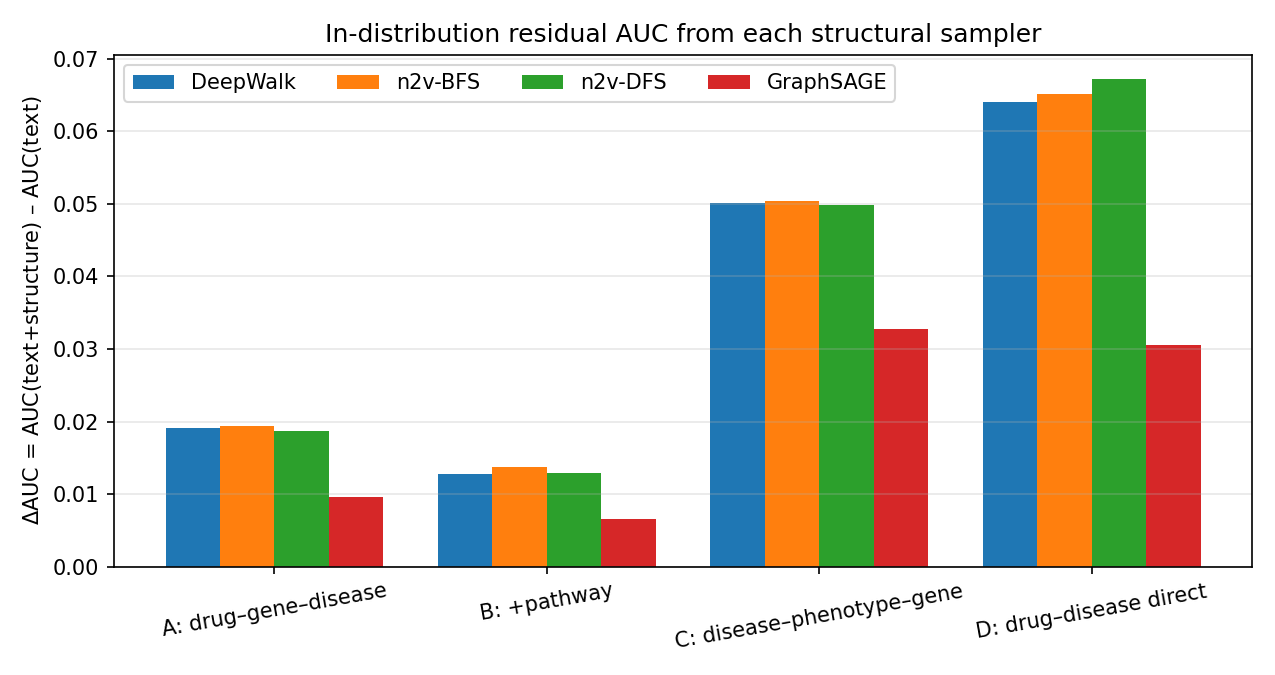
\includegraphics[width=\linewidth]{figures/fig_in_dist_auc_gap.png}
\caption{In-distribution AUC gap from structure, per (schema, embedder). The three random-walk embedders are statistically indistinguishable within each schema; GraphSAGE is consistently weakest.}
\label{fig:in-dist-bars}
\end{figure}

Two patterns are immediate. First, the AUC gap from structure anti-correlates with text-baseline strength: when text already classifies near-perfectly (Schemas A, B), structure adds only $+0.01$--$0.02$ AUC; when text is weaker (Schemas C, D), structure adds $+0.03$--$0.07$. Figure~\ref{fig:in-dist-bars} visualizes this pattern. Second, within each schema, the three random-walk embedders are statistically indistinguishable, while GraphSAGE consistently produces about half the AUC gap.

\subsection{Schema transfer: walk-based generalizes, aggregation does not}
\label{sec:transfer}

For each held-out schema we trained the DML nuisances on pairs pooled from the other three schemas, then evaluated on the held-out schema using its own embedder representations. Table~\ref{tab:transfer} reports out-of-distribution AUC; Figure~\ref{fig:transfer} visualizes the same.

\begin{table*}[h!]
\centering
\caption{Schema-transfer AUC. $\mathrm{AUC}_T$ is text-only trained on the three source schemas; remaining columns add each embedder's structural features on the held-out schema. Bold indicates AUC \emph{drops} below the text-only baseline.}
\label{tab:transfer}
\small
\begin{tabular}{l c c c c c}
\toprule
Held-out schema & $\mathrm{AUC}_T$ & DeepWalk & n2v-BFS & n2v-DFS & GraphSAGE \\
\midrule
A: drug--gene/protein--disease         & 0.994 & 0.997 & 0.997 & 0.997 & \textbf{0.979} \\
B: drug--gene/protein--pathway--disease & 0.995 & 0.997 & 0.998 & 0.996 & \textbf{0.989} \\
C: disease--phenotype--gene/protein    & 0.474 & 0.930 & 0.923 & 0.922 & 0.574 \\
D: drug--disease direct                & 0.954 & 0.983 & 0.982 & 0.985 & \textbf{0.768} \\
\bottomrule
\end{tabular}
\end{table*}

\begin{figure}[h!]
\centering
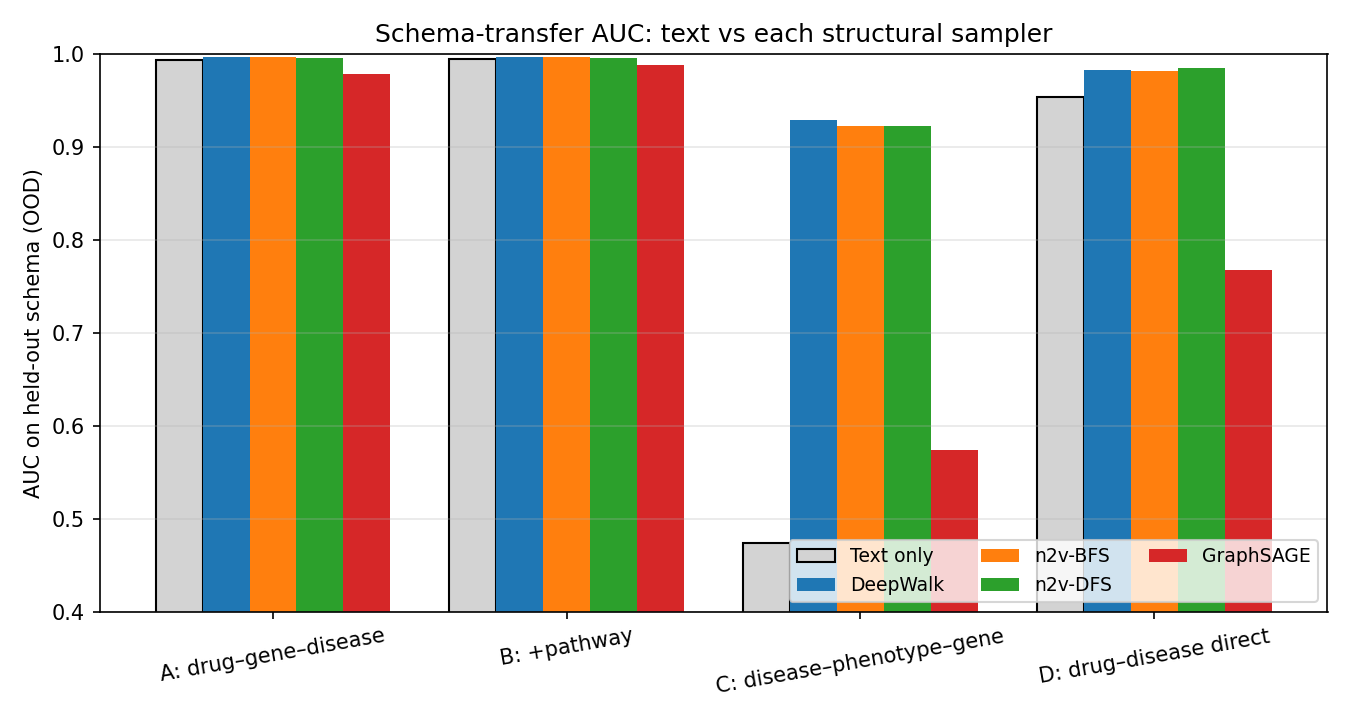
\includegraphics[width=\linewidth]{figures/fig_schema_transfer.png}
\caption{Schema-transfer AUC. Light-gray bars: text-only baseline trained on the three source schemas. Colored bars: same nuisance plus each embedder's structural features on the held-out schema. Walk-based embedders improve over text in every schema; GraphSAGE drops below text in three of four.}
\label{fig:transfer}
\end{figure}

Three observations. First, walk-based embedders transfer universally: all twelve (held-out schema, walk-based embedder) entries have $\mathrm{AUC} \geq \mathrm{AUC}_T$. Second, GraphSAGE fails to transfer in three of four schemas, with the catastrophic case on Schema D where AUC drops from $0.954$ (text alone) to $0.768$ (text + transferred GraphSAGE). Aggregation-based features are schema-specific. Third, when text breaks, structure carries the signal: on Schema C, text trained on the drug-related source schemas predicts disease--phenotype--gene associations at $\mathrm{AUC} = 0.474$, indistinguishable from random, while random-walk embeddings rescue prediction to $\mathrm{AUC} \approx 0.93$. Although the three random-walk embedders are indistinguishable in-distribution, node2vec-DFS is consistently the strongest transferer for the drug-related schemas (B and D); the BFS/DFS distinction emerges only under distribution shift.

\section{Conclusion}

Across four PrimeKG schemas and four structural embedders, graph structure adds residual predictive value beyond a Word2Vec text baseline in every (schema, embedder) combination, but the magnitude of that value is governed almost entirely by the strength of the text baseline: when text already classifies near-perfectly, structure adds little; when text is weaker, structure adds substantially more. Within a schema, the three random-walk embedders are statistically indistinguishable, so probe-level distinctions between proximity, BFS, and DFS biases collapse in-distribution.

The qualitative picture changes under schema shift. Walk-based embeddings transfer universally and, in the most extreme case, recover prediction from random ($\mathrm{AUC} = 0.474$) to $\mathrm{AUC} \approx 0.93$ when text generalization fails entirely. GraphSAGE fails to transfer in three of four schemas. We interpret this as evidence that walk-based structural features encode schema-invariant biological primitives, while parametric neighborhood aggregation encodes schema-specific patterns. For practitioners building knowledge-graph retrieval systems that must generalize across query types or biomedical sub-domains, this is a strong argument for walk-based structural representations.

\section{Limitations}

We use a fixed Word2Vec text encoder; stronger encoders such as SBERT or biomedical LLMs would shift the text baseline upward and likely shrink the residual AUC gap from structure. We use a single negative-sampling strategy (degree-matched random); harder negatives might change the absolute AUC numbers but, we conjecture, not the qualitative pattern of walk-vs-aggregation transfer. Our DML point estimate $\bar\tau$ exhibits calibration noise at small sample sizes; we mitigate this by relying on AUC-based permutation tests as the primary significance statistic. Finally, all results are on PrimeKG; generalization to other biomedical knowledge graphs (Hetionet, BioKG) is future work.

\bibliographystyle{icml202}
\begin{thebibliography}{99}
\bibitem[Chandak et al.(2023)]{primekg2023} Chandak, P., Huang, K., and Zitnik, M. \newblock Building a knowledge graph to enable precision medicine. \newblock \emph{Scientific Data}, 10(67), 2023.
\bibitem[Chernozhukov et al.(2018)]{dml2018} Chernozhukov, V., Chetverikov, D., Demirer, M., Duflo, E., Hansen, C., Newey, W., and Robins, J. \newblock Double/debiased machine learning for treatment and structural parameters. \newblock \emph{The Econometrics Journal}, 21(1):C1--C68, 2018.
\bibitem[Grover \& Leskovec(2016)]{node2vec} Grover, A. and Leskovec, J. \newblock node2vec: Scalable feature learning for networks. \newblock In \emph{KDD}, 2016.
\bibitem[Hamilton et al.(2017)]{graphsage} Hamilton, W. L., Ying, R., and Leskovec, J. \newblock Inductive representation learning on large graphs. \newblock In \emph{NeurIPS}, 2017.
\bibitem[Hogan et al.(2021)]{hogan2021} Hogan, A., et al. \newblock Knowledge graphs. \newblock \emph{ACM Computing Surveys}, 54(4):1--37, 2021.
\bibitem[Hu et al.(2024)]{grag2024} Hu, Y., et al. \newblock GRAG: Graph retrieval-augmented generation. \newblock arXiv:2405.16506, 2024.
\bibitem[Huang et al.(2023)]{huang2023} Huang, J., et al. \newblock Can LLMs effectively leverage graph structural information: When and why. \newblock arXiv:2309.16595, 2023.
\bibitem[Lewis et al.(2020)]{lewis2020rag} Lewis, P., et al. \newblock Retrieval-augmented generation for knowledge-intensive NLP tasks. \newblock In \emph{NeurIPS}, 2020.
\bibitem[Mikolov et al.(2013)]{word2vec} Mikolov, T., Sutskever, I., Chen, K., Corrado, G., and Dean, J. \newblock Distributed representations of words and phrases and their compositionality. \newblock In \emph{NeurIPS}, 2013.
\bibitem[Perozzi et al.(2014)]{deepwalk} Perozzi, B., Al-Rfou, R., and Skiena, S. \newblock DeepWalk: Online learning of social representations. \newblock In \emph{KDD}, 2014.
\bibitem[Wu et al.(2024)]{stark2024} Wu, S., et al. \newblock STaRK: Benchmarking LLM retrieval on textual and relational knowledge bases. \newblock In \emph{NeurIPS Datasets and Benchmarks}, 2024.
\bibitem[Yu et al.(2025)]{graphflow2025} Yu, J., et al. \newblock Can knowledge-graph-based retrieval augmented generation really retrieve what you need? \newblock In \emph{NeurIPS}, 2025.
\bibitem[Yue et al.(2025)]{mor2025} Yue, Z., et al. \newblock Mixture of structural-and-textual retrieval over text-rich graph knowledge bases. \newblock In \emph{Findings of ACL}, 2025.
\end{thebibliography}

\end{document}